%%%%%%%%%%%%%%%%%%%%%%%%
% Compile with XeLaTeX %
%%%%%%%%%%%%%%%%%%%%%%%%

\documentclass{beamer}\usepackage[]{graphicx}\usepackage[]{color}
% maxwidth is the original width if it is less than linewidth
% otherwise use linewidth (to make sure the graphics do not exceed the margin)
\makeatletter
\def\maxwidth{ %
  \ifdim\Gin@nat@width>\linewidth
    \linewidth
  \else
    \Gin@nat@width
  \fi
}
\makeatother

\definecolor{fgcolor}{rgb}{0.345, 0.345, 0.345}
\newcommand{\hlnum}[1]{\textcolor[rgb]{0.686,0.059,0.569}{#1}}%
\newcommand{\hlstr}[1]{\textcolor[rgb]{0.192,0.494,0.8}{#1}}%
\newcommand{\hlcom}[1]{\textcolor[rgb]{0.678,0.584,0.686}{\textit{#1}}}%
\newcommand{\hlopt}[1]{\textcolor[rgb]{0,0,0}{#1}}%
\newcommand{\hlstd}[1]{\textcolor[rgb]{0.345,0.345,0.345}{#1}}%
\newcommand{\hlkwa}[1]{\textcolor[rgb]{0.161,0.373,0.58}{\textbf{#1}}}%
\newcommand{\hlkwb}[1]{\textcolor[rgb]{0.69,0.353,0.396}{#1}}%
\newcommand{\hlkwc}[1]{\textcolor[rgb]{0.333,0.667,0.333}{#1}}%
\newcommand{\hlkwd}[1]{\textcolor[rgb]{0.737,0.353,0.396}{\textbf{#1}}}%
\let\hlipl\hlkwb

\usepackage{framed}
\makeatletter
\newenvironment{kframe}{%
 \def\at@end@of@kframe{}%
 \ifinner\ifhmode%
  \def\at@end@of@kframe{\end{minipage}}%
  \begin{minipage}{\columnwidth}%
 \fi\fi%
 \def\FrameCommand##1{\hskip\@totalleftmargin \hskip-\fboxsep
 \colorbox{shadecolor}{##1}\hskip-\fboxsep
     % There is no \\@totalrightmargin, so:
     \hskip-\linewidth \hskip-\@totalleftmargin \hskip\columnwidth}%
 \MakeFramed {\advance\hsize-\width
   \@totalleftmargin\z@ \linewidth\hsize
   \@setminipage}}%
 {\par\unskip\endMakeFramed%
 \at@end@of@kframe}
\makeatother

\definecolor{shadecolor}{rgb}{.97, .97, .97}
\definecolor{messagecolor}{rgb}{0, 0, 0}
\definecolor{warningcolor}{rgb}{1, 0, 1}
\definecolor{errorcolor}{rgb}{1, 0, 0}
\newenvironment{knitrout}{}{} % an empty environment to be redefined in TeX

\usepackage{alltt}

  % Beamer settings
  \usetheme{CambridgeUS}
  \usecolortheme{seagull}
  \usefonttheme{professionalfonts}
  \usefonttheme{serif}
  \setbeamertemplate{bibliography item}{}

  % Packages and settings
  \usepackage{fontspec}
    \setmainfont{Charis SIL}
  \usepackage[style=apa, backend=biber]{biblatex}
    \addbibresource{References.bib}
  \usepackage{hyperref}
    \hypersetup{colorlinks=true, allcolors=blue}
  \usepackage{siunitx}
    \sisetup{group-minimum-digits=4,
             group-separator={,},
             detect-all}
  \usepackage{tabularx}
    \newcolumntype{Y}{>{\raggedleft\arraybackslash}X}

  % Document information
  \title[Using LMs for variety comparisons]{Using language models for holistic language variety comparisons}
  \author{Joshua McNeill}
  \institute{University of Georgia}
  \date{9 October 2021}

  % New commands
  \newcommand{\orth}[1]{$\langle$#1$\rangle$}
  \newcommand{\lexi}[1]{\textit{#1}}
  \newcommand{\gloss}[1]{`#1'}
  \newcommand{\corp}[1]{\texttt{#1}}
  \newcommand{\hlight}[1]{\textcolor{red}{#1}}
\IfFileExists{upquote.sty}{\usepackage{upquote}}{}
\begin{document}


  \begin{frame}
    \titlepage
    \tiny{
      Data and code available at \url{https://osf.io/9cjpw/}.
    }
  \end{frame}

  \begin{frame}
    \tableofcontents[hideallsubsections]
  \end{frame}

  \AtBeginSection[]{
    \begin{frame}
      \tableofcontents[currentsection,
                       hideallsubsections]
    \end{frame}
  }

  \section{Distinguishing between varieties}
    \begin{frame}{Past studies}
      \begin{columns}
        \column{0.65\textwidth}
          \begin{enumerate}
            \item \alert{Atlases in dialectology} used many linguistic features, often lexical \parencite{gillieron_atlas_1902, wenker_sprach-atlas_2020}
            \item \alert{Modern studies} have focused on a handful of socially salient variables \parencite{dubois_verbal_2003, eckert_phonetics_2017, rickford_addressee-_1994}
            \item \alert{Recent online dialectology} returns to including many lexical items \parencite{eisenstein_identifying_2014, grieve_mapping_2018, pavalanathan_audience-modulated_2015}
          \end{enumerate}
        \column{0.35\textwidth}
      \end{columns}
    \end{frame}

    \begin{frame}{Research question}
      Given these limits:
      \begin{enumerate}
        \item Dialectology > Many but only \alert{lexical} features
        \item Sociolinguistics > \alert{Few} but diverse socially salient variables
      \end{enumerate}
      Can language models be used to capture many diverse linguistic features to more holistically quantify the difference between language varieties?
    \end{frame}

  \section{Language models (LMs)}
    \begin{frame}{Basic idea: $n$-gram LMs}
      \begin{block}{Europarl \parencite{koehn_europarl:_2009}}
        \corp{\input{./data/corpora/europarl_eg_lines.tex}}
      \end{block}
      \begin{columns}
        \column{0.5\textwidth}
          \begin{tabular}{l r}
            Word Bigram     & Tokens \\
            \hline
            Madam President & 1 \\
            President can   & 1 \\
            can you         & 1 \\
            you tell        & 1 \\
            tell me         & 1 \\
            me why          & 1 \\
            \ldots         & \ldots \\
            $bigram_n$      & $tokens_n$
          \end{tabular}
        \column{0.5\textwidth}
        \begin{tabular}{l r}
          Character 4-gram & Tokens \\
          \hline
          mada             & 1 \\
          adam             & 1 \\
          dam\_            & 1 \\
          am\_p            & 1 \\
          m\_pr            & 1 \\
          \_pre            & 1 \\
          \ldots           & \ldots \\
          $4gram_n$        & $tokens_n$
        \end{tabular}
      \end{columns}
    \end{frame}

    % \begin{frame}[t]{Uses}
    %   LMs constitute frequency distributions that can be compared to distributions constructed from new documents for classification \\
    %   \only<1>{
    %     \begin{center}
    %       \begin{tabular}{l r r r}
    %         $n$-gram & English LM & French LM & New document \\
    %         \hline
    %         wordBiDiffeG[1, "ngram"]  & wordBiDiffeG[1, "x"]  & wordBiDiffeG[1, "y"]  & 0 \\
    %         wordBiDiffeG[2, "ngram"]  & wordBiDiffeG[2, "x"]  & wordBiDiffeG[2, "y"]  & 0 \\
    %         wordBiDiffeG[3, "ngram"]  & wordBiDiffeG[3, "x"]  & wordBiDiffeG[3, "y"]  & 0 \\
    %         wordBiDiffeG[4, "ngram"]  & wordBiDiffeG[4, "x"]  & wordBiDiffeG[4, "y"]  & 0 \\
    %         wordBiDiffeG[5, "ngram"]  & wordBiDiffeG[5, "x"]  & wordBiDiffeG[5, "y"]  & 0 \\
    %         wordBiDiffeG[6, "ngram"]  & wordBiDiffeG[6, "x"]  & wordBiDiffeG[6, "y"]  & 0 \\
    %         wordBiDiffeG[7, "ngram"]  & wordBiDiffeG[7, "x"]  & wordBiDiffeG[7, "y"]  & 0 \\
    %         wordBiDiffeG[8, "ngram"]  & wordBiDiffeG[8, "x"]  & wordBiDiffeG[8, "y"]  & 1 \\
    %         wordBiDiffeG[9, "ngram"]  & wordBiDiffeG[9, "x"]  & wordBiDiffeG[9, "y"]  & 0 \\
    %         wordBiDiffeG[10, "ngram"] & wordBiDiffeG[10, "x"] & wordBiDiffeG[10, "y"] & 0 \\
    %       \end{tabular}
    %     \end{center}
    %   }
    %   \only<2>{
    %     Some tasks LMs have been used for:
    %     \begin{enumerate}
    %       \item Email spam classification \parencite{dada_machine_2019}
    %       \item News article topic classification
    %       \item Opinion classification \parencite{minaee_deep_2021}
    %       \item Language variety identification \parencite{bouamor_madar_2019, zampieri_findings_2017}
    %       \item And much more...
    %     \end{enumerate}
    %   }
    % \end{frame}

  \section{Methods}
    \begin{frame}{Data}
      The Europarl corpus \parencite{koehn_europarl:_2009}
      \begin{enumerate}
        \item Transcriptions of speeches from proceedings of the European Union dating back to 1996
        \item Parallel corpus (i.e., speeches translated into several languages)
        \item \num{50263238} words in English
        \item \num{52562008} words in French
        \item Well controlled for speech style and topic
      \end{enumerate}
      \begin{block}{Excerpt}
        \corp{\input{./data/corpora/europarl_excerpt.tex}}
      \end{block}
    \end{frame}

    \begin{frame}{LMs used}
      Training data:
      \begin{enumerate}
        \item English transcriptions vs French transcriptions
        \item 1st half of the English transcriptions vs 2nd half of the English transcriptions
        \item 1st half of the French transcriptions vs 2nd half of the French transcriptions
      \end{enumerate}
      The following LMs were constructed from each training set following \textcite{duvenhage_short_2019}:
      \begin{columns}
        \column{0.5\textwidth}
          \begin{enumerate}
            \setcounter{enumi}{3}
            \item Word $n$-gram LMs
            \begin{itemize}
              \item[$\to$] unigram and bigram
            \end{itemize}
          \end{enumerate}
        \column{0.5\textwidth}
          \begin{enumerate}
            \setcounter{enumi}{4}
            \item Character $n$-gram LMs
            \begin{itemize}
              \item[$\to$] bigram, 4-gram, and 6-gram
            \end{itemize}
          \end{enumerate}
      \end{columns}
    \end{frame}

    \begin{frame}{Analysis}
      To quantify the difference between varieties:
      \begin{enumerate}
        \item \alert{KL divergence}
        \begin{itemize}
          \item Range from 0 (no similarity) to $\infty$ (very similar)
        \end{itemize}
        \item Cosine similarity
        \begin{itemize}
          \item Range from -1 (opposite) to 0 (perpendicular) to 1 (identical)
        \end{itemize}
      \end{enumerate}
    \end{frame}

  \section{Results}
    \begin{frame}{Collated LMs}
      \begin{center}

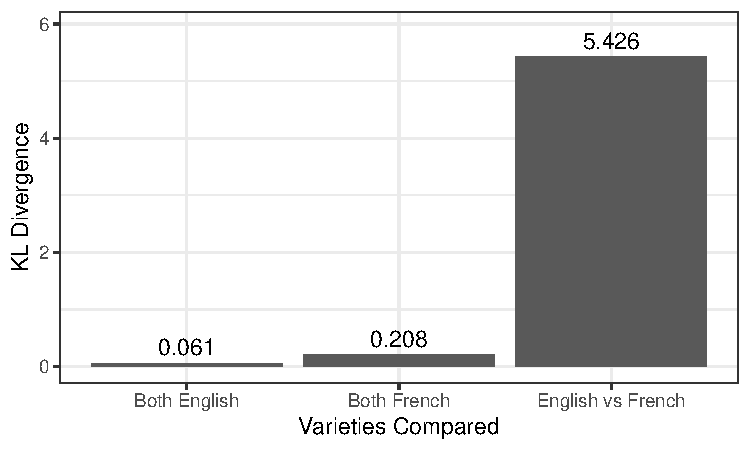
\includegraphics[width=\maxwidth]{figure/graphKLall-1} 

      \end{center}
    \end{frame}

    \begin{frame}{By LM type}
      \begin{center}

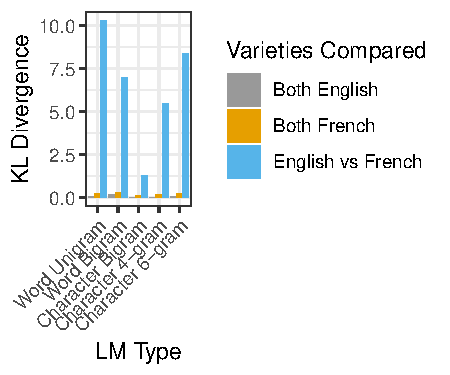
\includegraphics[width=\maxwidth]{figure/graphKLlinglevs-1} 

      \end{center}
    \end{frame}

    \begin{frame}{Character bigrams}
      \begin{columns}
        \column{0.35\textwidth}
          \begin{tabular}{l l}
            \multicolumn{2}{c}{10 Most Frequent} \\
            \hline
            English                                 & French \\
            \hline
            \hlight{e \_} & \hlight{e \_} \\
            \_ t          & \hlight{s \_} \\
            th            & \_ d \\
            \hlight{s \_} & es \\
            \_ a          & \_ l \\
            he            & \hlight{on} \\
            \hlight{t \_} & \hlight{t \_} \\
            n \_          & en \\
            in            & de \\
            \hlight{on}  & nt
          \end{tabular}
        \column{0.65\textwidth}
          Some matches are spurious
          \begin{enumerate}
            \item \lexi{on} is a preposition in English but a subject pronoun in French
            \item Words ending in \orth{t}, \orth{s}, or \orth{e} are common in both languages, but only \orth{s} is likely to have a shared meaning (i.e., plurality)
          \end{enumerate}
          Character bigrams arguably do not carry enough linguistically distinguishing information
      \end{columns}
    \end{frame}

    \begin{frame}{Capturing the lexicon: Word unigrams}
      \begin{columns}
        \column{0.4\textwidth}
          \begin{tabular}{l l}
            \multicolumn{2}{c}{5 Most Frequent} \\
            \hline
            English                                  & French \\
            \hline
            the            & de \\
            of            & la \\
            to            & et \\
            and            & le \\
            in            & à \\
            \hline
            Eng Half 1                               & Eng Half 2 \\
            \hline
            \hlight{the} & \hlight{the} \\
            \hlight{of} & \hlight{of} \\
            \hlight{to} & \hlight{to} \\
            \hlight{and} & \hlight{and} \\
            \hlight{in} & \hlight{in} \\
          \end{tabular}
        \column{0.6\textwidth}
          Matches are as expected
          \begin{enumerate}
            \item No matches between English and French
            \item Everything matches between English and English
          \end{enumerate}
          Function words are given greater weight
      \end{columns}
    \end{frame}

    \begin{frame}{Capturing syntax: Word bigrams}
      \begin{columns}
        \column{0.5\textwidth}
          \begin{tabular}{l l}
            \multicolumn{2}{c}{5 Most Frequent} \\
            \hline
            English                                  & French \\
            \hline
            of the            & de la \\
            in the            & à la \\
            to the            & et de \\
            the European            & que nous \\
            on the            & Monsieur le \\
            \hline
            Eng Half 1                              & Eng Half 2 \\
            \hline
            \hlight{of the} & \hlight{of the} \\
            \hlight{in the} & \hlight{in the} \\
            \hlight{to the} & \hlight{to the} \\
            \hlight{the European} & \hlight{the European} \\
            \hlight{on the} & \hlight{on the} \\
          \end{tabular}
        \column{0.5\textwidth}
          This is lexical rather than syntactic
          \begin{enumerate}
            \setcounter{enumi}{2}
            \item \lexi{of the} = \lexi{de la} : P Det
            \item \lexi{in the}/\lexi{to the} = \lexi{à la} : P Det
          \end{enumerate}
          Training on a PoS tagged corpus would overcome this
          \begin{enumerate}
            \setcounter{enumi}{4}
            \item Can be tagged manually or automatically
          \end{enumerate}
      \end{columns}
    \end{frame}

    \begin{frame}{Capturing morphology: Character 4-grams}
      \begin{columns}
        \column{0.4\textwidth}
          \begin{tabular}{l l}
            \multicolumn{2}{c}{5 Most Frequent} \\
            \hline
            English                                       & French \\
            \hline
            \_ the              & \_ de \_ \\
            the \_              & \_ la \_ \\
            \_ of \_            & tion \\
            \_ to \_            & ent \_ \\
            and \_              & ion \_ \\
            \hline
            Eng Half 1                                    & Eng Half 2 \\
            \hline
            \hlight{\_ the}   & \hlight{\_ the} \\
            \hlight{the \_}   & \hlight{the \_} \\
            \hlight{\_ of \_} & \hlight{\_ of \_} \\
            \hlight{\_ to \_} & \hlight{\_ to \_} \\
            \hlight{and \_}   & \hlight{and \_} \\
          \end{tabular}
        \column{0.6\textwidth}
          Function words are captured most frequently but also derivational morphemes in French
          \begin{enumerate}
            \item \lexi{ion}, \lexi{tion}, and \lexi{ent}
            \item Only the form of the morphemes is contrasted
          \end{enumerate}
      \end{columns}
    \end{frame}

    \begin{frame}{Capturing morphology: Character 6-grams}
      \begin{columns}
        \column{0.4\textwidth}
          \begin{tabular}{l l}
            \multicolumn{2}{c}{5 Most Frequent} \\
            \hline
            English                                      & French \\
            \hline
            \_ that \_            & ement \_ \\
            \_ of th              & ation \_ \\
            n the \_              & \_ de la \\
            of the                & de la \_ \\
            f the \_              & \_ dans \_ \\
            \hline
            Eng Half 1                                   & Eng Half 2 \\
            \hline
            \hlight{\_ that \_} & \hlight{\_ that \_} \\
            \hlight{\_ of th}   & \hlight{\_ of th} \\
            \hlight{n the \_}   & \hlight{n the \_} \\
            \hlight{of the}     & \hlight{of the} \\
            \hlight{f the \_}   & \hlight{f the \_} \\
          \end{tabular}
        \column{0.6\textwidth}
          \only<1>{
            Again, function words are the most frequent items captures but also some derivational morphemes in French
            \begin{enumerate}
              \item \lexi{ment} and \lexi{tion}
              \item For both function words and morphemes, additional context is captured
              \item Again, only forms are contrasted
            \end{enumerate}
          }
          \only<2>{
            This really captures orthographic differences and, to some extent, phonetic differences
            \begin{enumerate}
              \setcounter{enumi}{1}
              \item Training character $n$-gram LMs on a phonetic transcription would better capture phonetic differences
            \end{enumerate}
          }
      \end{columns}
    \end{frame}

  \section{Discussion}
    \begin{frame}{Limitations}
      \begin{enumerate}
        \item Special care needs to be given to the LMs used
        \item Special care needs to be given to the corpora used
        \begin{itemize}
          \item This method likely won't work well with small corpora either
        \end{itemize}
        \item This method gives no great value to particularly salient features
      \end{enumerate}
    \end{frame}

    \begin{frame}{What's next}
      \begin{enumerate}
        \item Explore using PoS tagging to better capture syntax in the LMs
        \item Look into the impact of using corpora of different sizes
        \item Apply the method to data that has already been analyzed with traditional variationist methods
      \end{enumerate}
    \end{frame}

  \section{References}
    \printbibliography

    \begin{frame}{Bonus slides}
      \begin{center}

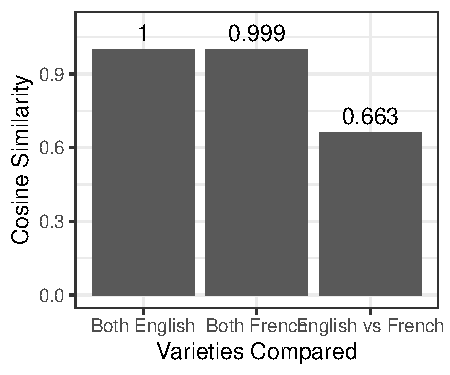
\includegraphics[width=\maxwidth]{figure/graphCosSimall-1} 

      \end{center}
    \end{frame}

    \begin{frame}{Bonus Slides}
      \begin{center}

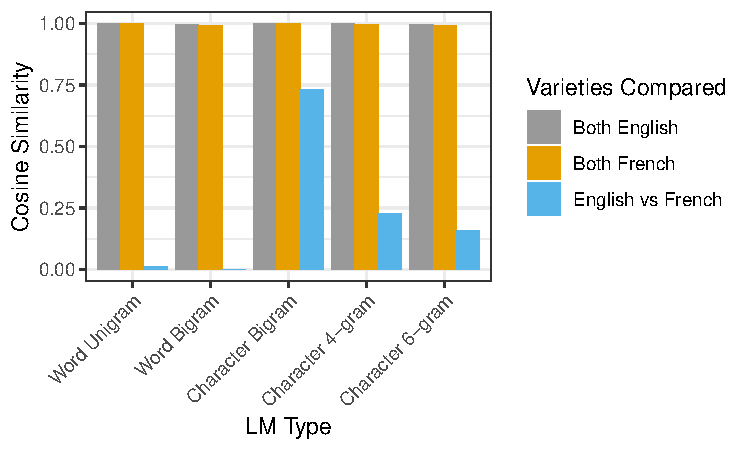
\includegraphics[width=\maxwidth]{figure/graphCosSimlinglevs-1} 

      \end{center}
    \end{frame}

\end{document}
